% !TEX program = xelatex
% 在本目录运行 XeLaTeX。评分截图 autograder.png 与本文件同目录。
% 如需合并手写答题页，将扫描件保存为同目录的 Q8手写.pdf，再重新编译。
\documentclass[UTF8,fontset=fandol,a4paper,11pt]{ctexart}
\usepackage[left=23mm,right=23mm,top=20mm,bottom=21mm]{geometry}
\usepackage{amsmath,amssymb,booktabs,tabularx,array}
\usepackage{graphicx,xcolor,listings,pdfpages}
\usepackage[hidelinks]{hyperref}
\hypersetup{pdftitle={人工智能 PJ2：强化学习实验报告},pdfauthor={陈家龙、刘俊彦}}
\setlength{\parindent}{2em}
\setlength{\parskip}{2pt}
\setlength{\emergencystretch}{2em}
\linespread{1.08}
\setlength{\abovedisplayskip}{6pt plus 2pt minus 2pt}
\setlength{\belowdisplayskip}{6pt plus 2pt minus 2pt}
\setlength{\tabcolsep}{6pt}
\ctexset{
  section={format=\large\bfseries,beforeskip=12pt,afterskip=5pt},
  subsection={format=\normalsize\bfseries,beforeskip=8pt,afterskip=3pt}
}
\pagestyle{plain}
\newcommand{\code}[1]{\texttt{#1}}
\newcolumntype{Y}{>{\raggedright\arraybackslash}X}
\lstset{
  language=Python,
  basicstyle=\ttfamily\footnotesize,
  columns=fullflexible,
  keepspaces=true,
  showstringspaces=false,
  backgroundcolor=\color{black!4},
  keywordstyle=\bfseries,
  commentstyle=\color{black!65},
  aboveskip=5pt,
  belowskip=5pt,
  xleftmargin=7pt,
  xrightmargin=7pt,
  framexleftmargin=7pt,
  framexrightmargin=7pt
}
\begin{document}

\begin{center}
  {\LARGE\bfseries 人工智能 PJ2：强化学习实验报告}\par
  \vspace{4pt}
\end{center}
\vspace{-2pt}
\begin{center}
  \begin{tabularx}{0.95\linewidth}{>{\centering\arraybackslash}p{28mm} >{\centering\arraybackslash}p{38mm} Y}
    \toprule
    姓名 & 学号 & 分工 \\
    \midrule
    \rule{0pt}{2mm} 陈家龙 & 24300980041 & Q2、Q4、Q6 \\
    \rule{0pt}{7mm} 刘俊彦 & 24300980021 & Q1、Q3、Q5、Q7、Q8、撰写报告 \\
    \bottomrule
  \end{tabularx}
\end{center}

\section{实验环境与课上核心算法}

实验在 Windows、Python 3.13.9 环境下运行。课上实现位于 \code{Agents/Coursework} 下的 \code{value\_iteration\_agents.py} 和 \code{qlearning\_agents.py}。

\subsection{Q1：值迭代}

\code{ValueIterationAgent} 从零值函数出发，根据模型的奖励和转移概率计算
\[
  Q_k(s,a)=R(s,a)+\gamma\sum_{s'}P(s'\mid s,a)V_k(s'),
  \qquad V_{k+1}(s)=\max_{a\in A(s)}Q_k(s,a).
\]
每轮将结果写入新的 \code{Counter}，全轮结束后才替换 \code{self.values}。真正的终止状态价值为零，奖励格仍可执行 \code{exit} 以取得奖励。策略从当前值函数向前看一步，取 Q 值最大的合法动作，无合法动作时返回 \code{None}。

\begin{lstlisting}
for _ in range(self.iterations):
    new_values = util.Counter()
    for state in self.mdp.getStates():
        if self.mdp.isTerminal(state):
            new_values[state] = 0
        else:
            action_values = []
            for action in self.mdp.getPossibleActions(state):
                q_value = self.computeQValue(state, action)
                action_values.append(q_value)
            new_values[state] = max(action_values)
    self.values = new_values
\end{lstlisting}

默认 \code{BookGrid} 中，起点值在第 5 轮为 0，在第 100 轮约为 0.490684。第 5 轮完成后的策略已选择向北，因为 \code{computeQValue} 会在 $V_5$ 基础上再做一次单步前瞻。

\subsection{Q2：表格型 Q-Learning}

\code{QLearningAgent} 用 \code{Counter} 保存 $(s,a)$ 的 Q 值，未访问动作的初值为零。它遍历全部合法动作并通过 \code{getQValue} 查询，因而也能复用在 Q6 的近似智能体中。当前代码在并列时保留合法动作列表中最先出现的动作。无合法动作时返回 \code{(None, 0.0)}，此时更新目标只有即时奖励。

每次观察到 $(s,a,r,s')$ 后，用样本目标 $r+\gamma V(s')$ 更新对应的表项。若下一状态有合法动作，$V(s')$ 取这些动作中最大的 Q 值。
\begin{lstlisting}
Q = self.getQValue(state, action)
alpha = self.alpha
gamma = self.discount
next_value = self.getValue(nextState)
target = reward + gamma * next_value
self.qvalues[(state, action)] = Q + alpha * (target - Q)
\end{lstlisting}

\newpage
\section{课后实验实现}

\subsection{Q3：\texorpdfstring{$\epsilon$}{ε}-贪婪策略}

\code{getAction} 先检查合法动作，再以概率 $\epsilon$ 从所有合法动作中均匀抽样，以概率 $1-\epsilon$ 调用当前贪婪策略。若有 $m$ 个合法动作，利用分支所选动作的总概率为 $1-\epsilon+\epsilon/m$，因为探索时也可能抽到它。
\begin{lstlisting}
if not legalActions:
    return None
if util.flipCoin(self.epsilon):
    action = random.choice(legalActions)
else:
    action = self.getPolicy(state)
return action
\end{lstlisting}

在无转移噪声的 \code{BookGrid} 上，以 $\alpha=0.5$、$\gamma=0.9$ 各训练 100 局，每组从同一随机种子 50020 开始。$\epsilon$ 为 0.1、0.3、0.9 时，训练期平均折扣回报依次为 0.5372、0.4613、$-0.0101$。关闭探索和学习后，各组的单局贪婪测试回报均为 0.59049。

\subsection{Q4：折扣网格的最优策略}

\code{analysis.py} 的五个函数返回 $(\gamma,\text{noise},\text{livingReward})$。用指定噪声计算策略，再沿策略指定方向行走以检查预期路线。表中 N、E、S 分别表示北、东、南，到达奖励格后执行 \code{exit}。

\begin{center}
  \small
  \renewcommand{\arraystretch}{1.18}
  \begin{tabularx}{\linewidth}{@{}l c l Y@{}}
    \toprule
    子题 & 参数组 & 路线 & 预期结果 \\
    \midrule
    (a) & $(0.2,0,-1)$   & E,E,N             & 近端 $+1$，贴近悬崖 \\
    (b) & $(0.2,0.2,-1)$ & N,N,N,E,E,S,S     & 近端 $+1$，绕开悬崖 \\
    (c) & $(0.9,0,0)$    & E,E,E,E,N         & 远端 $+10$，贴近悬崖 \\
    (d) & $(0.9,0.2,0)$  & N,N,N,E,E,E,E,S,S & 远端 $+10$，绕开悬崖 \\
    (e) & $(0.01,0,1000)$ & N,N,N，随后持续向北 & 到达上边界后原地循环 \\
    \bottomrule
  \end{tabularx}
\end{center}

(a)、(b) 的低折扣因子削弱远期回报，负生存奖励使绕路付出代价。(c)、(d) 提高折扣并将生存奖励设为零，远端 $+10$ 的回报足以补偿较长路线。在 (b)、(d) 中，噪声 0.2 使每个垂直于指令方向的偏移各有 0.1 的概率，贴崖向东时可能滑入 $-10$ 区域。(e) 每步的高生存奖励使持续行动优于离开。

\begin{lstlisting}
def question2d():
    answerDiscount = 0.9
    answerNoise = 0.2
    answerLivingReward = 0
    return answerDiscount, answerNoise, answerLivingReward
\end{lstlisting}

\subsection{Q5：Q-Learning 与勇者斗恶龙}

\code{HeroQAgent} 复用 Q2 的更新和 Q3 的动作选择。其 \code{getAction} 调用父类选择动作，再用 \code{doAction(state, action)} 记录当前状态和动作供奖励回传。评分器以 $\epsilon=0.05$、$\alpha=0.2$、$\gamma=0.8$ 在 \code{smallGrid} 上训练 2,000 局，之后将 $\epsilon$ 和 $\alpha$ 置零并测试 100 局。实测 100 局全胜，平均得分 500.60，达到 70 局的满分门槛。
\begin{lstlisting}
def getAction(self, state):
    action = QLearningAgent.getAction(self, state)
    self.doAction(state, action)
    return action
\end{lstlisting}

\newpage
\subsection{Q6：值近似与特征设计}

\textbf{Q6.1 基础算法。}\code{ApproximateQAgent} 将 Q 值表示为权重与稀疏特征的内积。每次转移先计算同一个时序差分误差 $\delta$，再更新当前特征向量中出现的权重。
\[
  Q_w(s,a)=\sum_i w_i f_i(s,a),\qquad
  \delta=r+\gamma V_w(s')-Q_w(s,a),\qquad
  w_i\gets w_i+\alpha\delta f_i(s,a).
\]
使用 \code{IdentityExtractor} 时，每个 $(s,a)$ 只激活其专属的值为 1 的特征。在学习参数相同的条件下，其更新退化为表格型 Q-Learning。
\begin{lstlisting}
def getQValue(self, state, action):
    features = self.featExtractor.getFeatures(state, action)
    return self.weights * features

def update(self, state, action, nextState, reward: float):
    features = self.featExtractor.getFeatures(state, action)
    Q = self.getQValue(state, action)
    next_value = self.getValue(nextState)
    alpha = self.alpha
    gamma = self.discount
    target = reward + gamma * next_value
    delta = target - Q
    for feature, value in features.items():
        self.weights[feature] += alpha * delta * value
\end{lstlisting}

\textbf{Q6.2 特征设计。}\code{StudentFeatureExtractor} 以 \code{SimpleExtractor} 为基础，保留常数偏置 0.1 和候选位置到最近可达金币的 BFS 距离（除以地图面积，再除以 10）。候选位置由当前位置和待评估动作确定。危险计数 $D$ 统计可在一步内到达候选位置的恶龙，纳入虚弱计时为 0 或 1 的个体。候选位置有宝剑时，拾剑会让恶龙进入虚弱状态，因此将 $D$ 置零。金币指示只在 $D=0$ 时启用，并另设拾剑指示。特征计算仅读取游戏状态。

\begin{lstlisting}
danger = 0
for dragon in state.getDragonStates():
    if dragon.weakenedTimer <= 1:
        neighbors = Actions.getLegalNeighbors(dragon.getPosition(), walls)
        if next_position in neighbors:
            danger += 1
if takes_sword:
    danger = 0
features['#-of-dragons-1-step-away'] = danger / 10.0
features['collects-coin'] = float(
    danger == 0 and state.getCoins()[next_position[0]][next_position[1]]) / 10.0
features['takes-sword'] = float(takes_sword) / 10.0
\end{lstlisting}

特征实验使用 \code{mediumGrid}、\code{smallClassic} 和 \code{mediumClassic}，每张地图独立训练三次。每次使用新智能体训练 2,000 局，再测试 100 局。训练参数固定为 $\alpha=0.2$、$\gamma=0.99$、$\epsilon=0.05$，对手为随机恶龙，每局最多 900 次勇者行动。测试阶段停止探索和学习。

基础算法通过五个用例，获 3/3。三张地图的测试胜局依次为 300/300、245/300 和 270/300，合计 815/900（90.56\%），达到 80\% 的满分门槛，特征设计获 3/3。\code{smallClassic} 的胜率最低，为 81.67\%。

\newpage
\subsection{Q7：深度强化学习}

\code{dqn\_utils.py} 中的 \code{EpsilonScheduler.value} 按已采集的环境步数 $t$ 计算探索率。将 $t/D$ 裁剪到 $[0,1]$ 后，对起始探索率和结束探索率进行线性插值。第 $D$ 步后保持结束值。
\begin{lstlisting}
progress = min(1.0, max(0.0, step / self.decay_steps))
return self.start + (self.end - self.start) * progress
\end{lstlisting}

\code{ReplayBuffer} 用限长队列保存原始转移。加入新转移时，若队列已满则自动淘汰最早的一条。\code{sample} 对当前经验均匀无放回采样，经验仍保留在队列中。
\begin{lstlisting}
def __init__(self, capacity):
    if int(capacity) <= 0:
        raise ValueError('Replay capacity must be positive')
    self.buffer = deque(maxlen=capacity)

def add(self, transition):
    self.buffer.append(transition)

def sample(self, batch_size):
    return random.sample(list(self.buffer), batch_size)

def __len__(self):
    return len(self.buffer)
\end{lstlisting}

课程提供的 Double DQN 训练流程由在线网络选择下一状态的最优合法动作，由目标网络估值。实验验证了探索率调度与经验回放两个必做组件，选做的 Q7.3 未运行。

\section{自动评分结果}

在 \code{PJ2} 目录下执行 \code{python autograder.py --no-graphics}，Q1--Q7 共获 25/25。图~\ref{fig:autograder} 截取自本次运行的原始日志。Q8 手写答题页另附。

\begin{figure}[!h]
  \centering
  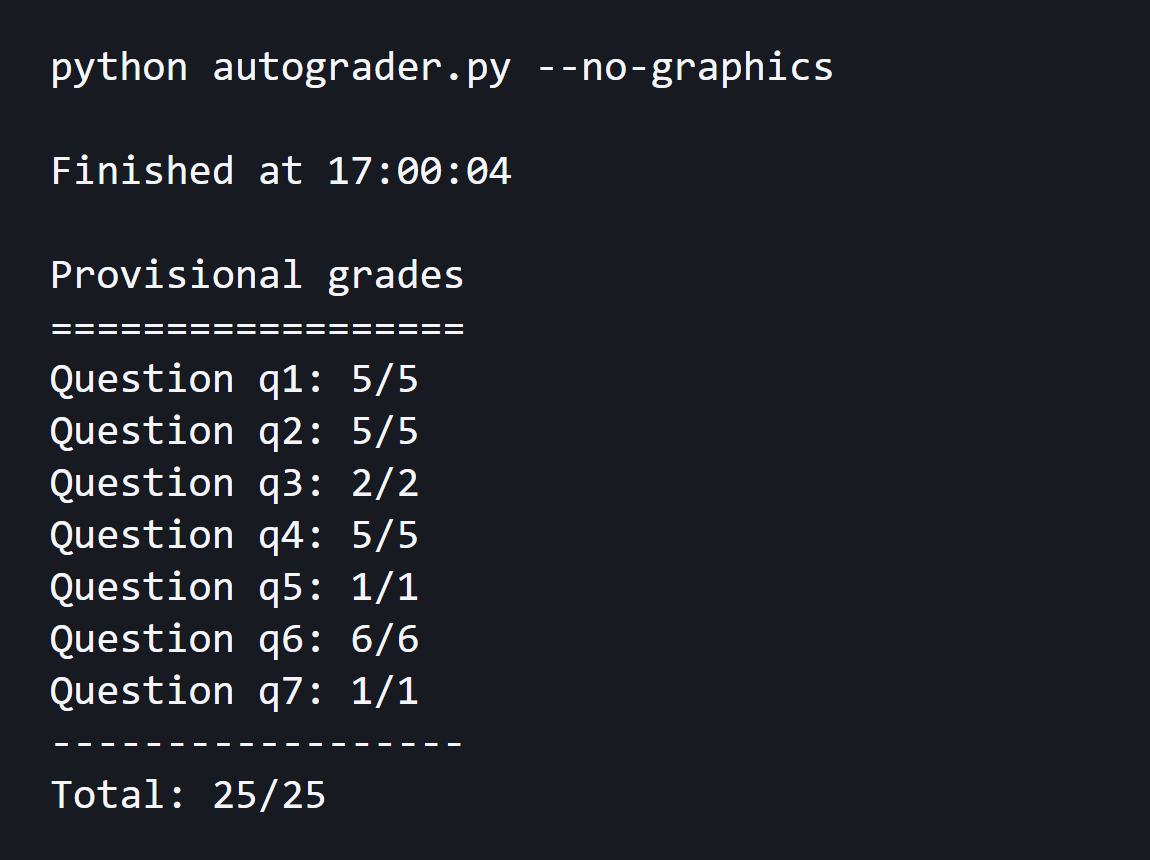
\includegraphics[width=0.64\linewidth]{autograder.png}
  \caption{自动评分汇总}
  \label{fig:autograder}
\end{figure}

\IfFileExists{Q8手写.pdf}{\clearpage\includepdf[pages=-,pagecommand={}]{Q8手写.pdf}}{}
\end{document}
